\documentclass[letterpaper,12pt,oneside]{article}
% JACARANDA — FINAL PROJECT | UNAM FI, COMPILERS, TEAM 01
\usepackage[top=1in,left=1.25in,right=1.25in,bottom=1in]{geometry}
\usepackage[T1]{fontenc}
\usepackage[utf8]{inputenc}
\usepackage[english]{babel}
\usepackage{lmodern,graphicx,float,booktabs,tabularx,array,amsmath,amssymb,enumitem,microtype,needspace}
\usepackage{tikz}
\usetikzlibrary{arrows.meta,positioning,shapes.geometric}
\usepackage[hidelinks]{hyperref}
\graphicspath{{figs/}}
\definecolor{jacPurple}{HTML}{7553A6}
\definecolor{jacDark}{HTML}{51356F}
\definecolor{jacGreen}{HTML}{237A60}
\definecolor{jacRed}{HTML}{B45055}
\tikzset{jbox/.style={draw=jacPurple,rounded corners=3pt,fill=jacPurple!5,text=jacDark,align=center,font=\small,minimum height=11mm,text width=8cm}, jarrow/.style={->,thick,draw=jacPurple}}
\setlength{\parindent}{0pt}
\setlength{\parskip}{.55em}
\setlength{\emergencystretch}{2em}
\renewcommand{\arraystretch}{1.15}
% Screenshots must be real, tightly cropped photographs of the running application.
\newcommand{\evidence}[3]{\begin{figure}[H]\centering
\IfFileExists{figs/#1}{\includegraphics[width=.94\textwidth,height=.34\textheight,keepaspectratio]{#1}}{\fbox{\parbox[c][3.8cm][c]{.84\textwidth}{\centering\textbf{Screenshot pending}\\[5pt]Save a real cropped capture as \\ \texttt{\detokenize{#1}} in the \texttt{figs/} folder.}}}
\caption{#2}\label{fig:#3}\end{figure}}
\begin{document}
\begin{titlepage}
\setlength{\parindent}{0pt}\setlength{\parskip}{0pt}
\begin{center}
\vfill

\includegraphics[width=4.2cm]{UNAM_LOGO2.png}\\[.65cm]
{\Huge\bfseries National Autonomous University of Mexico}\\[.35cm]
{\Large Faculty of Engineering}\\[.85cm]
{\large Computer Engineering}\\[.28cm]
{\large Compilers}\\[.9cm]
{\Huge\bfseries JACARANDA}\\[.25cm]
{\LARGE\bfseries FINAL PROJECT REPORT}\\[.3cm]
{\Large C-like Educational Interpreter}\\[.65cm]
{\large\bfseries Team 01 -- Group 5}\\[.25cm]
{\large Semester 2027-1}\\[.75cm]
\begin{tabular}{ll}
\textbf{Team members:} & Aguilar Lara Ericka -- 321227122 \\
& Bautista Reyes Sofía -- 321103891 \\
& Cruz Basilio Ximena Carolina -- 321116424 \\
& Garibay Zamorano Josué Benjamín -- 321206105 \\
& Jardón Marín Rodrigo -- 321240693 \\
\end{tabular}
\vfill
Mexico City, Mexico. November 2026
\end{center}
\end{titlepage}
\begingroup\small\setlength{\parskip}{0pt}\tableofcontents\endgroup\clearpage
\section{Introduction}
\subsection{Problem Statement}
The first version of Jacaranda identified lexical units, while the second delivery verified grammatical structures and selected semantic rules. Both could report errors, but neither executed the source instructions. The final assignment asks for a compiler, interpreter or assembler that processes a source instruction set and displays its results. To meet that requirement using the team's previous concepts, Jacaranda has been extended into an \textbf{educational interpreter of a C-like subset}. It is not a native-code compiler and does not claim complete compatibility with C.

\subsection{Motivation}
Interpreting the statements after validating them makes the distinction between identifying a program and executing it explicit. The project now connects syntax recognition, semantic checking and runtime behavior, while keeping error categories separate. A grammar-based parser also offers an opportunity to compare the manual recursive-descent method from the preceding delivery with a parser generated by a library.

\subsection{Objectives}
\textbf{General objective.} Implement a C-like educational interpreter capable of reading source code, validating grammar and semantic constraints, and executing supported instructions with visible results.

\textbf{Specific objectives.}
\begin{itemize}[leftmargin=1.5em]
\item Replace manual parsing in the final execution pipeline with a library-generated LALR parser.
\item Define a restricted C-like grammar, generate a parse tree, and perform static semantic checks.
\item Execute variables, arithmetic and logical operations, functions, conditional branches and loops.
\item Support nested scopes, typed values and parameter checking.
\item Report syntax, semantic and runtime errors and protect against unbounded execution.
\item Integrate terminal and graphical interfaces and provide reproducible tests.
\end{itemize}

\section{Theoretical Framework}
\subsection{Interpreter and Compiler}
A compiler generally translates source code into another representation or executable form before it runs. An interpreter performs the program's operations using an execution engine, typically after some parsing and validation. Jacaranda follows the latter approach: it reads the source, generates a parse tree and traverses it to carry out the supported instructions. It does not emit native machine code.

\subsection{Library-Generated LALR Parsing}
The first delivery used RPLY for lexical recognition. The second used a manually implemented top-down recursive-descent parser. For the final delivery, the execution pipeline uses \textbf{Lark 1.3.1} with a \textbf{LALR} parsing configuration. The grammar is declared separately in a \texttt{.lark} file and defines both lexical elements and syntactic productions. In contrast with recursive descent, the parser's recognition engine is provided by the library. Semantic checks and interpretation remain implemented in project code.

\subsection{Semantic Analysis and Symbol Tables}
Before execution, the analyzer checks identifiers, declared types, duplicate variables, function existence and parameters. A hierarchy of symbol tables represents nested scopes. For expressions, the analyzer determines types and checks compatibility. The final version adds argument-count and argument-type checking, extending the limits of the previous SDT implementation. The rules are educational simplifications and are not a formal implementation of all C conversion rules.

\subsection{Runtime Execution and Error Handling}
The execution engine evaluates expressions, updates variable values and follows control flow. It uses bounded execution steps and call depth to prevent simple infinite loops or unbounded recursion from continuing forever. Errors are presented with source-line information and distinguished by their stage. These safeguards improve robustness, although the interpreter is not designed as a secure sandbox for untrusted programs.

\section{Development}
\subsection{Project Architecture}
The final implementation is organized in a separate \texttt{final\_project/} directory to preserve the lexer, parser, diagrams and reports from earlier submissions. Its main modules are the grammar, execution engine, semantic analyzer, command-line entry point and Tkinter graphical interface.

\begin{figure}[H]\centering
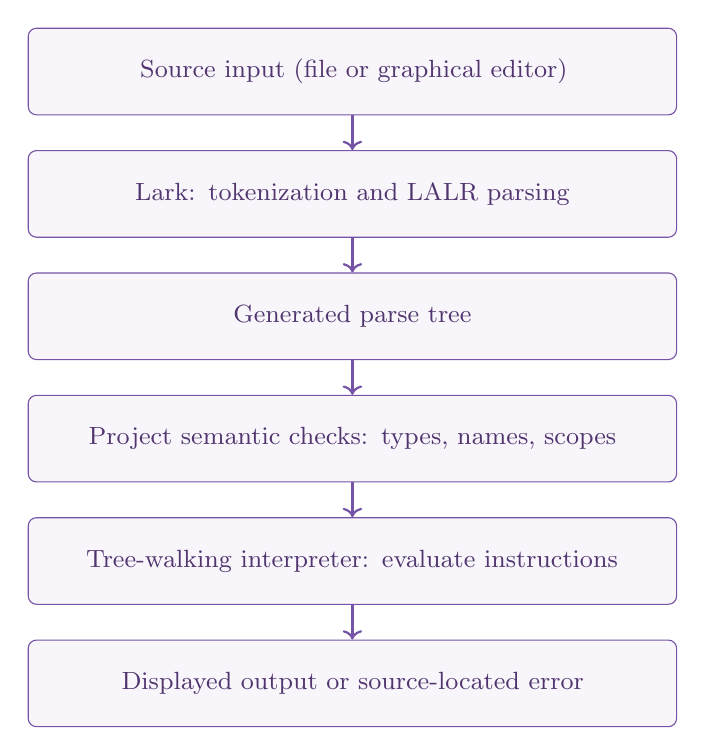
\begin{tikzpicture}[node distance=.44cm]
\node[jbox] (a) {Source input (file or graphical editor)};
\node[jbox,below=of a] (b) {Lark: tokenization and LALR parsing};
\node[jbox,below=of b] (c) {Generated parse tree};
\node[jbox,below=of c] (d) {Project semantic checks: types, names, scopes};
\node[jbox,below=of d] (e) {Tree-walking interpreter: evaluate instructions};
\node[jbox,below=of e] (f) {Displayed output or source-located error};
\foreach \x/\y in {a/b,b/c,c/d,d/e,e/f}{\draw[jarrow] (\x)--(\y);}
\end{tikzpicture}
\caption{Final interpreter execution pipeline. The interpreter runs only after parsing and static checks succeed.}\label{fig:architecture}
\end{figure}

\subsection{Grammar and Language Subset}
The grammar accepts variable declarations with optional initialization, assignments, arithmetic, comparison and logical expressions, function definitions and calls, typed parameters, return statements, blocks and the control structures \texttt{if/else}, \texttt{while}, \texttt{for} and \texttt{do/while}. It also supports printing statements and increment/decrement. Operator levels define precedence and grouping, while the parser library produces a structured representation to be consumed by later stages.

\begin{table}[H]\centering\small
\caption{Main features of the supported educational language.}
\begin{tabularx}{\textwidth}{>{\bfseries}p{.31\textwidth} X}\toprule
Language feature & Implemented behavior\\\midrule
Types & Integer, float, double, boolean and character variables; functions may return void.\\
Expressions & Arithmetic, modulo, comparison, logical operations, unary operators and parentheses.\\
Statements & Declarations, assignments, printing, increments and returns.\\
Control flow & Conditional branches, while, for and do-while loops.\\
Functions & Typed parameters, calls, returns and bounded recursion.\\
Scope & Nested local environments and shadowing.\\
\bottomrule\end{tabularx}\end{table}

The project deliberately excludes pointers, arrays, structures, standard headers, full standard-library behavior, native compilation and complete C semantics. Division yields floating-point results even for integer operands, which is an explicit project-specific rule.

\subsection{Semantic Verification}
The static stage records functions and their signatures, then checks statements before runtime execution. It verifies declaration-before-use, uniqueness within a scope, assignment compatibility, operand types, condition types, return compatibility and function arguments. This allows a syntactically valid program to fail semantic validation before any instruction is executed, including errors in unreachable branches within the supported checks.

\subsection{Execution Engine}
Once validation succeeds, the interpreter evaluates top-level statements and calls \texttt{main()} when present. A stack of execution environments stores typed values, allowing function calls, nested blocks and recursive execution. Loops repeatedly evaluate their conditions and bodies; conditional statements select their appropriate branch. Print instructions append the evaluated text to the visible output. This is the principal change from the Parser \& SDT project: successful analysis now leads to \textbf{observable program execution}.

\subsection{Application Integration and Packaging}
The final version has both a terminal interface and a graphical interface with actions for execution, parsing, tree inspection, file opening and saving. In the prepared GitHub integration, these components are placed in \texttt{final\_project/src/}, while previous modules remain in the repository's original \texttt{src/} directory. This minimizes merge conflicts and preserves the results of the earlier assignments. Lark is the active lexer/parser of the final interpreter; RPLY is retained only for the earlier submissions.

\section{Results}
\subsection{Testing Method}
The prepared final implementation includes 15 example source files covering normal execution, arithmetic precedence, functions, conditionals, loops, errors, shadowing, parameter checks and execution limits. Six automated tests were executed in this working environment and passed. The following screenshots must be taken directly on the team's computer, showing only the program's input/output area or a tightly cropped terminal. The spaces below are intentionally not filled with fabricated screenshots.

\subsection{Basic Execution}
The valid basic program verifies that the parser accepts the input, that semantic checks succeed, and that the interpreter displays the result of the printing instruction.
\evidence{01_basic_run.png}{Real execution of the basic example, including output.}{basic}

\subsection{Functions and Parameters}
A second example verifies that function calls evaluate their arguments, create a local environment and return a value to the caller. The analyzer also rejects incompatible or missing arguments according to the declared function signature.
\evidence{02_functions.png}{Execution of a function with typed parameters and a return value.}{functions}

\subsection{Conditional Statements and Loops}
The loop example executes an accumulation and repetition instructions. Its expected printed values are 15, 0, 1 and 2, in that order. This demonstrates that the final project \textit{executes} loops rather than merely recognizing their syntax.
\evidence{03_loops.png}{Execution of the loop example and its visible output.}{loops}

\subsection{Error Categories}
The examples also distinguish grammatical errors, type errors, runtime errors and missing functions. The system reports the appropriate stage and source line, so an error discovered before execution does not produce successful runtime output.
\evidence{04_syntax_error.png}{Parsing error reported for a malformed program.}{syntax}
\evidence{05_semantic_error.png}{SDT error after successful parsing.}{semantic}
\evidence{06_runtime_error.png}{Runtime error such as division by zero or an exceeded execution limit.}{runtime}

\subsection{Graphical Interface}
The new Tkinter interface contains a source editor and analysis/output panel. It provides actions to run the source, check parsing, inspect the generated tree, and load or save code. Its visual operation should be verified on the team's desktop before submission.
\evidence{07_gui.png}{Final interpreter graphical interface with an executed example.}{gui}

\begin{table}[H]\centering\small
\caption{Representative prepared examples and behaviors.}
\begin{tabularx}{\textwidth}{>{\ttfamily}p{.37\textwidth} X}\toprule
Example & Purpose / expected result\\\midrule
01\_hello.c & Basic execution with printed output.\\
02\_functions.c & Function definition and call.\\
03\_loops.c & Loop execution and numeric accumulation.\\
04\_conditionals.c & Branch selection.\\
05\_semantic\_error.c & Semantic type error before execution.\\
06\_syntax\_error.c & Syntactic error.\\
08\_runtime\_error.c & Runtime failure handling.\\
13\_wrong\_arguments.c & Parameter-count or type validation.\\
15\_infinite\_loop.c & Execution step limit.\\
\bottomrule\end{tabularx}\end{table}

\section{Repository}
The final interpreter was prepared for integration into the public project repository:\\
\url{https://github.com/ErickaAgui/unam.fi.compilers.g5.01}

The project manager must commit the new folder, review the changes and verify the public main branch before submitting the repository link. The final assignment requires the repository, a report and a presentation. The required submission date is December 1, 2026.

\section{Conclusions}
The final stage changes Jacaranda from a system that only recognizes and verifies code into an educational interpreter that also executes it. Using Lark to generate the parser reduces the amount of handwritten parsing logic and allows the team to focus on semantic checks and runtime behavior. The project retains the conceptual stages developed in earlier assignments and illustrates how lexical recognition, syntax, semantic verification and execution depend on each other.

The supported language remains a deliberately restricted C-like subset, so the team should describe its actual features and limitations during the demonstration. The automated tests validate important paths, but complete visual verification and real cropped screenshots from the final desktop application remain necessary before the report can be considered submission-ready.

\begin{thebibliography}{9}
\bibitem{assignment} Universidad Nacional Autónoma de México, Facultad de Ingeniería, \emph{Final Project: Compiler/Interpreter/Assembler}, Compilers, Group 5, 2026. Course assignment supplied by the instructor.
\bibitem{aho} A. V. Aho, M. S. Lam, R. Sethi, and J. D. Ullman, \emph{Compilers: Principles, Techniques, and Tools}, 2nd ed. Pearson, 2006.
\bibitem{lark} Lark contributors, \emph{Lark Parser Documentation}. Available: \url{https://lark-parser.readthedocs.io/}.
\bibitem{repo} Team 01, \emph{Jacaranda Project Repository}. Available: \url{https://github.com/ErickaAgui/unam.fi.compilers.g5.01}.
\end{thebibliography}
\end{document}
